\documentclass{beamer}
\usepackage[dvips]{epsfig}
\usepackage[dvips]{graphicx}
\usepackage[utf8]{inputenc}
\usepackage{verbatim}
\usepackage{graphicx}
\usepackage{moreverb}
\let\verbatiminput=\verbatimtabinput
%\documentclass[xcolor=DarkRed]{beamer}
%\usepackage{beamerthemesplit}
\usetheme{CambridgeUS}
%\documentclass[xcolor=DarkRed]{beamer}

\title{``\'Emile Durkheim''} 
\subtitle{Sistemas y Organizaciones}
\author{Cristi\'an Maureira, Rodrigo Fern\'andez}
\titlegraphic{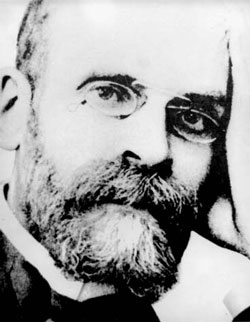
\includegraphics[width=2.5cm]{images/foto}}
%\logo{\includegraphics[width=1.5cm]{images/alma_logo}}


\date{\today}

\begin{document}
\frame{\titlepage}
\frame{\tableofcontents}

\section{Contexto Hist\'orico}
\frame{
\frametitle{Contexto Hist\'orico}
\begin{center}
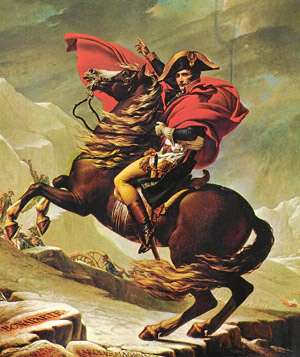
\includegraphics[height=3.5cm]{images/napoleon}
\end{center}
\begin{itemize}
	\item \textbf{El segundo imperio (1852-1870) de Napoleon}
	\begin{itemize}
		\item Su gobierno se apoy\'o en el clero, en la alta burgues\'ia y en la poblaci\'on rural.
		\item Pol\'itica empe\~nada en realzar el prestigio del pa\'is y del r\'egimen.
		\item En pol\'itica exterior se inici\'o la conquista del Senegal, se penetr\'o en Argelia y se intervino en Indochina.
		\item El r\'egimen se basaba en la prosperidad econ\'omica, pero \'esta entr\'o en crisis en 1870.
	\end{itemize}
\end{itemize}
}
\frame{
\frametitle{Contexto Hist\'orico}
\begin{center}
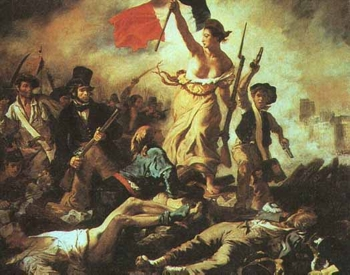
\includegraphics[height=3cm]{images/revolucion}
\end{center}
\begin{itemize}
	\item \textbf{La tercera rep\'ublica}
	\begin{itemize}
		\item La comuna revolucionaria de Par\'is, que hab\'ia surgido aprovechando el vac\'io del poder (1871), fue aplastada.
		\item 1875: Se elabor\'o la constituci\'on de 1875, de car\'acter conservador.
		\item 1884: El movimiento obrero obtendr\'ia m\'as tarde la legalizaci\'on de los sindicatos. 
		\item 1902: El bloque de izquierdas triunf\'o en las elecciones.
		\begin{itemize}
			\item se separ\'o la Iglesia del estado (1905) y se difundi\'o la ense\~nanza laica.
			\item se intent\'o hacer frente a los problemas sociales mediante una legislaci\'on protectora de los trabajadores.
		\end{itemize}
	\end{itemize}
\end{itemize}

}

\section{Contexto Filos\'ofico}
%Cristian
\frame{
\frametitle{Contexto Filosófico}
\begin{itemize}
	\item El pensamiento filosófico francés del siglo XIX y principios del siglo XX está dominado por el positivismo de Comte.
	\item Coexisten otras corrientes de cierta importancia:
	\begin{itemize}
		\item Espiritualismo, de Alfredo Fouillée (1838-1912) y de Víctor Cousin (1892-1867)
		\item Neocriticismo de Carlos Renouvier (1815-1903).
	\end{itemize}
\end{itemize}
}

\frame{
\frametitle{Espiritualismo y Neocriticismo}
\begin{itemize}
	\item Espiritualismo, movimiento que sostiene como creencia principal que los expertos pueden hacer contacto con los espíritus de los muertos, aconsejándonos sobre problemas. Los espiritus existen y están en una realidad distinta y superior a la materia
	\item Neocriticismo, pensamiento que contempla las condiciones y posibilidades del conocimiento humano desde el punto de vista del criticismo kantiano.
	\begin{itemize}
		\item El Criticismo Kantiano, \emph{pretende establecer los límites del conocimiento cierto a través de una investigación sistemática de las condiciones del pensamiento.}
	\end{itemize}
\end{itemize}

}
\frame{
\frametitle{Comte y el Positivismo}
\begin{itemize}
	\item El único conocimiento auténtico es el conocimiento científico, y que tal conocimiento solamente puede surgir de la afirmación positiva de las teorías a través del método científico.
	\item Según la misma, todas las actividades filosóficas y científicas deben efectuarse únicamente en el marco del análisis de los hechos reales verificados por la experiencia.
\end{itemize}

}
\section{Biograf\'ia}
\frame{
\frametitle{Su Vida}

\begin{columns}
	\begin{column}{0.2\textwidth}
		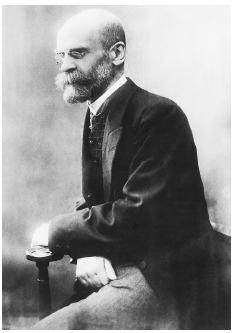
\includegraphics[width=2.5cm]{images/durkheim}
	\end{column}
	\begin{column}{0.8\textwidth}
		\begin{itemize}
			\item Épinal, Francia, 15 de abril 1858 — París, Francia, 15 de noviembre 1917
			\item Junto a Max Weber y Karl Marx, fue uno de los fundadores de la sociología moderna.
			\item Fundador de la 1ra revista dedicada a las ciencias sociales \emph{Année Sociologique}
			\item Hijo de un Rabino (8 generaciones)
			\item Influencias del Método Científico (Fen. Religiosos, provienen fact. sociales)
			\item Se convirtió al Catolicismo (influencias)
			\item Ecole Normale Superieure (3ra es la vencida)
		\end{itemize}
	
	\end{column}
\end{columns}
}
\frame{
\frametitle{Su Vida}

\begin{columns}
	\begin{column}{0.8\textwidth}
		\begin{itemize}
			\item Su generación fue una de las más brillantes del siglo XIX
			\begin{itemize}
				\item Jean Jaurès y Henri Bergson.
			\end{itemize}
			\item En 1887, es nombrado profesor de pedagogía y ciencia social de la Universidad de Burdeos.
			\item Fue el primero en enseñar Sociología en Francia.
			\item Como consecuencia de los pesares que le causó la muerte de su único hijo, falleció.
		\end{itemize}
	\end{column}
	\begin{column}{0.2\textwidth}
		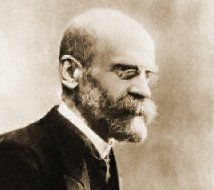
\includegraphics[width=2.5cm]{images/durkheim2}
	\end{column}
\end{columns}
}

\section{Obras}
%READY
%Cristian
\frame{
\frametitle{Obras Principales}
\begin{itemize}
	\item La Solidaridad Social
	\begin{itemize}
		\item \emph{"La División del Trabajo Social" (1893)}
		\item \emph{"La Solidaridad Social"}
	\end{itemize}
	\item \emph{El afincamiento de la sociología como ciencia autónoma}
	\begin{itemize}
		\item \emph{"Las Reglas del Método Sociológico" (1895)}
		\item \emph{"El Suicidio" (1897)}
	\end{itemize}
	\item Educación y Pedagogía
	\begin{itemize}
		\item \emph{"Educación" (publicado 1911)}
	\end{itemize}
	\item Teoría Política y Derecho
	\begin{itemize}
		\item \emph{"Física de las Costumbres y del Derecho" (póstuma 1950)}
	\end{itemize}
	\item La Moral
	\begin{itemize}
		\item \emph{"La Ciencia de la Moral en Alemania" (1887)}
		\item \emph{"La Determinación del Hecho Moral" (1906)}
		\item \emph{"Juicios de Valor y Juicios de Realidad" (1911)}
		\item \emph{"Introducción a la Moral"}
	\end{itemize}
	\item La Filosofía
	\begin{itemize}
		\item \emph{"Las Formas Elementales de la Vida Religiosa" (1912)}
	\end{itemize}
\end{itemize}
}

\section{Pensamientos}
%READY
%cristian
\frame{
\frametitle{Pensamientos de Durkheim}
\begin{itemize}
	\item \emph{Los Hechos Sociales}
	\item \emph{La División del Trabajo Social}
	\item \emph{Educación}
	\item \emph{Crimen}
	\item \emph{Ley}
	\item \emph{El Suicidio}
	\item \emph{Religión}
\end{itemize}
}
\frame{
%cristian
\frametitle{Los Hechos Sociales}
\begin{itemize}
	\item<1-> Sociología según Comte y Spencer
	\item<2-> Independencia Sociológica
	\item<3-> Fenómenos Sociales
	\item<4-> Técnicas Únicas
	\item<5-> Pero...¿Qué es un Hecho Social?
	\item<6-> \emph{"Modos de actuar, de pensar y de sentir exteriores al individuo y que poseen un poder de coerción en virtud del cual se imponen"}
\end{itemize}	
}
\frame
{
\frametitle{Características}
	\begin{enumerate}
		\item Exterioridad
		\item Coerción
		\item Colectividad
	\end{enumerate}
}
\frame
{
\frametitle{Uhm...¿y qué puedo concluir de todo ésto?}
\begin{itemize}
	\item Todo Rol que desempeñamos con nuestros pares, está dentro de un \emph{Hecho Social}.
	\item Sobre la coerción...la Conciencia Pública reprime todo acto que la ofenda.
	\item Sobre la colectividad...nos constituyen las creencias, tendencias...todas las prácticas de grupo!
	\item Condición Extra!
	\begin{itemize}
		\item Encarnarse en la psiquis de cada individuo en una sociedad, por lo tanto transformar la forma
		subjetiva se sentir determinados hechos.
	\end{itemize}
\end{itemize}
}

\frame{
\frametitle{La divisi\'on del Trabajo Social}
\begin{center}
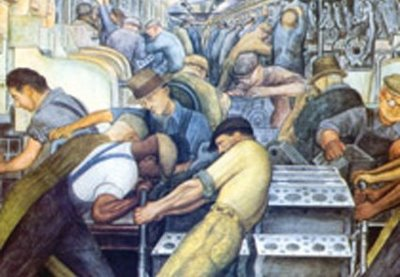
\includegraphics[height=3cm]{images/divisiontrabajo}
\end{center}
\begin{itemize}
	\item El problema de la \textbf{Solidaridad Social}.
	\item Opone la organizaci\'on de las sociedades arcaicas frente a la moderna.
	\item La diversificaci\'on del trabajo es la soluci\'on encontrada ante la escasez, producto del crecimiento demogr\'afico en un mismo espacio.
\end{itemize}
}
\frame{
\frametitle{La divisi\'on del Trabajo Social}
\begin{block}{En \textbf{Sociedades Primitivas}}
	\begin{itemize}
		\item Divisi\'on del trabajo es casi imperceptible.
		\item La comunidad es autosuficiente.
		\item Se habla de una ``\textbf{solidaridad mec\'anica}'':
		\begin{itemize}
			\item Solidaridad de la colectividad es muy estrecha. 
		\end{itemize}
		\item La conciencia colectiva pr\'acticamente anula a la individual.
	\end{itemize}
\end{block}
\begin{center}
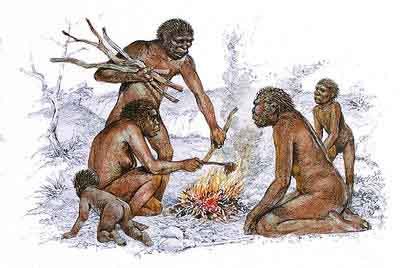
\includegraphics[height=3cm]{images/primitivas}
\end{center}
}
\frame{
\frametitle{La divisi\'on del Trabajo Social}
\begin{block}{Por el contrario, en \textbf{Sociedades Modernas}}
	\begin{itemize}
		\item Imprescindible la diversificaci\'on del trabajo para poder atender las necesidades de la colectividad.
		\item Estratifica a la sociedad acorde a sus funciones.
		\item Durkheim la llama una ``\textbf{solidaridad org\'anica}''.
	\end{itemize}
\end{block}
\begin{center}
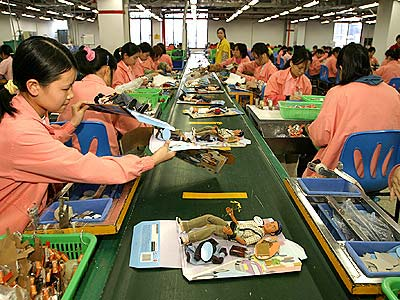
\includegraphics[height=3cm]{images/chinos}
\end{center}
}
\frame{
\frametitle{La divisi\'on del Trabajo Social}
\begin{alertblock}{}
	En las sociedades modernas, esta alta divisi\'on del trabajo conllevaba a un aumento de los estados de confusi\'on, lo cual provocaba un estado de ....
\end{alertblock}
\begin{center}

\includegraphics[height=2cm]{images/anomia}
\end{center}

\begin{block}{La \textbf{Anomia}}
	\begin{itemize}
		\item Carencia de solidaridad social.
		\item Se debe a una repentina ruptura del equilibrio social.
		\item Mal que sufre una sociedad a causa de la ausencia de reglas morales y reglas jur\'idicas.
	\end{itemize}
\end{block}
}


\frame{
\frametitle{Otros Pensamientos de Durkheim}
\begin{block}{Educaci\'on}
	Estudi\'o su importancia de su papel para evitar la anomia.
\end{block}
\begin{alertblock}{Funciones que esta cumpl\'ia:}
	\begin{itemize}
		\item Mejorar la solidaridad social
		\item Mantener el orden social
		\item Mantener la divisi\'on del trabajo
	\end{itemize}
\end{alertblock}
}
\frame{
\begin{block}{Ley y el Crimen}
	\begin{itemize}
		\item Distingi\'o sus diferencias entre las distintas sociedades:
		\begin{description}
			\item[En Sociedades Primitivas:] Ofensa para toda la sociedad, con una pena represiva (el criminal sufre un castigo).
			\item[En Sociedades Modernas:] Problema entre los involucrados, con una pena restitutiva (el criminal es responsable de reparar).
		\end{description}
	\end{itemize}
\end{block}
\begin{itemize}
	\item \textbf{Ley}
	\begin{itemize}
		\item Profundamente interesado en el estudio de la ley y sus efectos sociales en general.
		\item Fue de interes a la socilog\'ia por el hecho de poder revelar detalles sobre la naturaleza de la solidaridad.
	\end{itemize}

	\item \textbf{Crimen}
	\begin{itemize}
		\item Ve\'ia que el crimen era el abandono de las nociones convencionales.
		\item Dictaba que el crimen era ``un util preludio para las reformas''.
	\end{itemize}
\end{itemize}
}
\frame{
\frametitle{Otros Pensamientos de Durkheim}
\begin{block}{El Suicidio}
	\begin{itemize}
		\item Durkheim explora las diferentes tasas de suicidios entre Protestantes y Cat\'olicos.
		\item La socidad Cat\'olica poseia niveles normales de integraci\'on social.
		\item A pesar de sus limitaciones, su trabajo en el suicidio a influenciado diferentes exponentes.
		\begin{itemize}
			\item Suicidios Egoistas
			\item Suicidios Altruistas
			\item Suicidios Animos
			\item Suicidios Fatalistas
		\end{itemize}
	\end{itemize}
\end{block}
\begin{block}{Religi\'on}
	\begin{itemize}
		\item En el pasado, la religi\'on habia sido el cimiento de la sociedad.
		\item Mecanismo que fortalecia al orden social.
		\item Condenso las religiones en cuatro funciones mayores.
	\end{itemize}
\end{block}
}

\section{Conclusiones}
\frame{
\frametitle{Conclusiones}
\begin{itemize}
	\item La visi\'on de Durkheim de la sociedad marc\'o al pensamiento mundial en una manera que era
muy necesaria, dejar de lado todo tipo de prejuicios y emociones para generar un juicio imparcial y
racional de \'esta se volvio el pilar de la Sociolog\'ia, ciencia que hoy en dia se ha establecido como
una de las mas importantes de las Ciencias Sociales.
\end{itemize}
}
\frame{
\frametitle{Conclusiones}
\begin{itemize}
	\item A trav\'es de las ideas del autor, las empresas se pueden analizar con ``sangre fr\'ia'', extrapolan-
do las ideas de ``hechos sociales'' y ``estructura'' a organizaciones mas pequeñas. De esta manera se
puede entender mejor la forma de comportarse de algunas organizaciones que tienden
a la autodestrucci\'on o que logran surgir en ambientes altamente hostiles.
\end{itemize}
}
\frame{
\frametitle{Conclusiones}
\begin{itemize}
	\item Para el estudio y administraci\'on de empresas u organizaciones, el concepto de solidaridad desarrollado
por Durkheim es importante de recalcar. Vi\'endolo desde su punto de vista, cada organizaci\'on deber\'ia 
buscar una solidaridad mec\'anica entre sus miembros.
\end{itemize}
}

%\section{Cuestionario}
%\frame{
%\frametitle{Cuestionario}
%}

\end{document}
